%\documentclass[preprint,showpacs,preprintnumbers,superscriptaddress,prb,floatfix,aps]{revtex4-1}
\documentclass[twocolumn,showpacs,preprintnumbers,superscriptaddress,prb,floatfix,aps,10pt]{revtex4-1}

\usepackage{amsmath,amssymb}
\usepackage{graphicx,textcomp}
\usepackage{physics} % bra-ket
\usepackage{braket}  % over-write bra-ket
\usepackage{epstopdf}
\usepackage{subfigure}
\usepackage{xfrac} % nice frac
\usepackage{multirow} % multirow table

\usepackage[version=3]{mhchem}
\usepackage{siunitx}
\sisetup{
  separate-uncertainty,
  output-open-uncertainty=[
}


\usepackage{xcolor}
\definecolor{abm}{RGB}{190,220,170}
\usepackage{todonotes}
\presetkeys%
    {todonotes}%
    {inline,backgroundcolor=abm}{}
%
\newcommand{\abmei}[1]{\textcolor{orange}{ \bf [Antonio: #1] }}
\renewcommand{\vec}[1]{\ensuremath{\mathbf{#1}}}
\newcommand*{\ham}{\hat{H}}
\newcommand*{\class}{\mathcal{C}}
\newcommand*{\wignerD}{\mathbb{D}}%(R)
\newcommand*{\wignerDl}{D^{l}}%(R)
\newcommand*{\id}{\mathcal{E}}
\newcommand*{\zeromat}{0}
\newcommand*{\bloch}{\ket{\vec{k}, i\alpha}}
\newcommand*{\lowdin}{\ket{\vec{r}, i\alpha}}
\newcommand*{\x}{\times}
\newcommand*{\bondvec}{\vec{r}_{ij}}
\newcommand{\seitz}[2]{\{#1|#2\}}
\newcommand*{\nesting}{\chi(\vec{q})}

\begin{document}
\pagenumbering{arabic}

\title{VN ARPES}

\author{A. B. Mei}
\affiliation{Department of Materials Science and the Materials Research Laboratory
University of Illinois, 104 South Goodwin, Urbana, IL 61801}

\author{L. Hultman}
\affiliation{Department of Physics, Chemistry and Biology (IFM), Link\"oping University, SE-581 83, Link\"oping, Sweden.}

\author{I. Petrov}
\affiliation{Department of Materials Science and the Materials Research Laboratory
University of Illinois, 104 South Goodwin, Urbana, IL 61801}
\affiliation{Department of Physics, Chemistry and Biology (IFM), Link\"oping University, SE-581 83, Link\"oping, Sweden.}

\author{J. E. Greene}
\affiliation{Department of Materials Science and the Materials Research Laboratory
University of Illinois, 104 South Goodwin, Urbana, IL 61801}
\affiliation{Department of Physics, Chemistry and Biology (IFM), Link\"oping University, SE-581 83, Link\"oping, Sweden.}

\begin{abstract}

This highly-efficient basis is able to accurately reproduce both electronic band dispersion determined by ARPES and \emph{ab initio} density functional theory simulations with a minimal set of fourteen empirical fitting parameters.
\end{abstract}

\maketitle


%	
%	\begin{figure}[hbt,width=2]
%	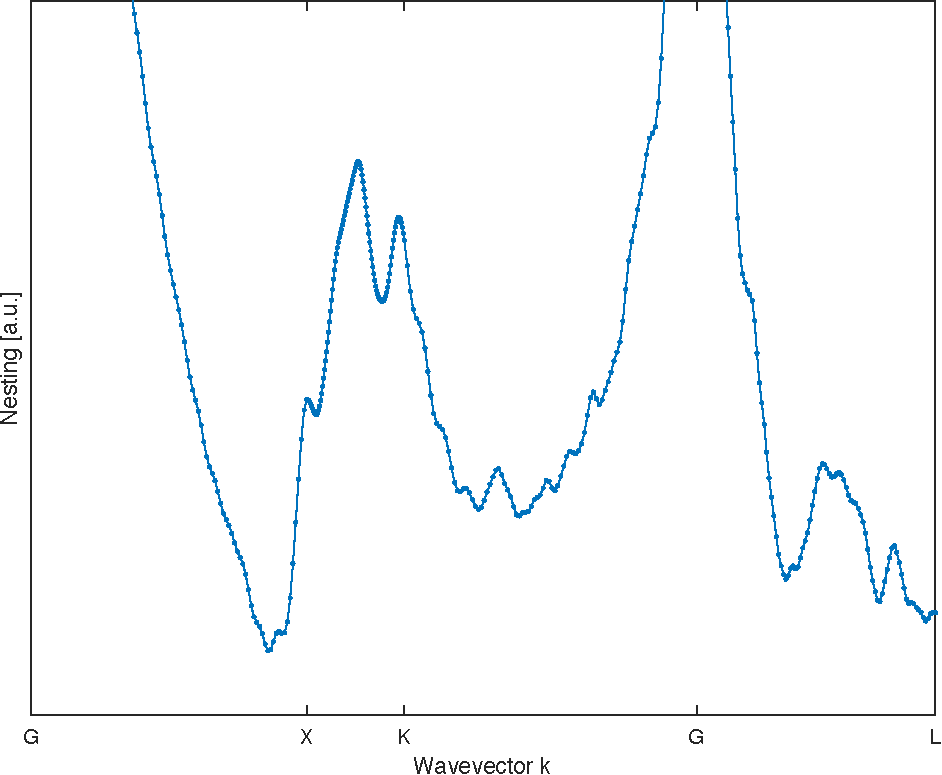
\includegraphics[width=0.47\textwidth]{Figure_2.pdf}
%	\caption[LRC circuit response.]{\label{fig:LR_circuit_IV} }
%	\end{figure}

\section{Calculation of Electronic Bands and Topological Properties}
The electronic band dispersion and topological properties of B1 NaCl-structure VN are computed using a minimal-basis orthogonal second-neighbor tight-binding model based upon V $d$ and N $p$ orbitals. 

Energy-momentum dispersion relations $E(\vec{k})$ are obtained by solving the secular equation
% CARDONA p 88 + HESS p 36
\begin{equation}
\label{eq:secular}
\left| \ham^{\alpha\beta}_{ij}(\vec{k}) - E(\vec{k})\delta_{\alpha\beta}\delta_{ij} \right| = 0
\end{equation}
%
associated with the time-independent Schrodinger equation 
%
\begin{equation}
\label{eq:schrodinger}
\hat{H}(\vec{k}) \ket{\psi} = E(\vec{k}) \ket{\psi}.
\end{equation}
%
The scripts on $\ham^{\alpha\beta}_{ij}(\vec{k})$ denote matrix elements of $\ham(\vec{k})$ with respect to wavevector $\vec{k}$ and orbitals $\alpha$ and $\beta$ centered on atoms $i$ and $j$; in Dirac notation, $\ham^{\alpha\beta}_{ij}(\vec{k}) = \braket{\vec{k},i\alpha | \ham | \vec{k},j\beta}$. $\delta$ represents Kronecker deltas and $|\cdot |$ indicates matrix determinant. Resulting tight-binding energy band dispersions are presented along high symmetry reciprocal space directions in Figure \ref{fig:dispersion}. For comparison, density functional theory calculations results obtained using the generalized gradient approximation are also plotted for comparison. The minimal tight binding basis efficiently and accurately reproduces the \emph{ab initio} dispersion, especially near the Fermi level. 

The Hamiltonian eigenfunctions $\ket{\psi}$ reside in the space spanned by linear combinations of $\bloch$ periodic Bloch sates. $\bloch$ is in turn defined through 
% KITTEL p 246
\begin{equation}
\label{eq:bloch}
\bloch = \frac{1}{\sqrt{N}} \sum_i e^{i\vec{r}_i\cdot\vec{k}} \lowdin, 
\quad
\alpha \equiv (l_\alpha,m_\alpha)
\end{equation}
as the Fourier transform of $\lowdin$, orthogonal atomic-like orbitals centered on atom $i$ and described by azimuthal and magnetic quantum numbers $l_\alpha$ and $m_\alpha$. Identification of the orbitals associated with each band is achieved by projecting the Hamiltonian eigenfunctions on symmetery-adapted Bloch basis functions $p$, $d_{t2g}$, and $d_{eg}$ and graphically represented in Figure \ref{fig:dispersion} by reducing the high-dimensional character space onto a one-dimensional linear color map. The three lowest bands display primarily $p$ character; the next three higher energy states consist predominately of $d_{t2g}$ orbitals; and the remaining two bands are chiefly comprised of $d_{eg}$ states.
%
\begin{figure}[h]
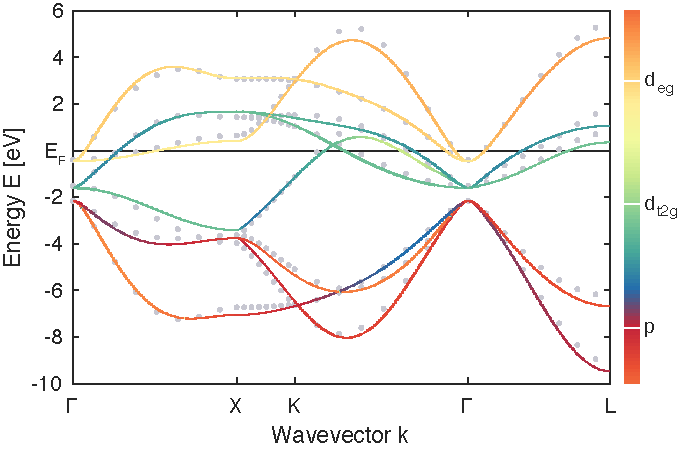
\includegraphics[width=0.47\textwidth]{Figure_1_bands.pdf}
\caption[LRC circuit response.]{\label{fig:dispersion} }
\end{figure}

The Fermi surface corresponds to the constant-energy manifold formed by the intersection of bands with the Fermi level $E_F$. For VN, a maximum of five bands cross $E_F$. The individual surfaces generated by each band is presented in Figures \ref{fig:fermi_surface}(a)-(e) and the combined surfaces are shown in Figure \ref{fig:fermi_surface}(f); the coloring scheme is identical to that of Figure \ref{fig:dispersion}. With increasing distance from $\Gamma$ the zone-center, the character of Fermi-level states evolves from $d_{eg}$ to $d_{t2g}$. 
%
\begin{figure}[h]
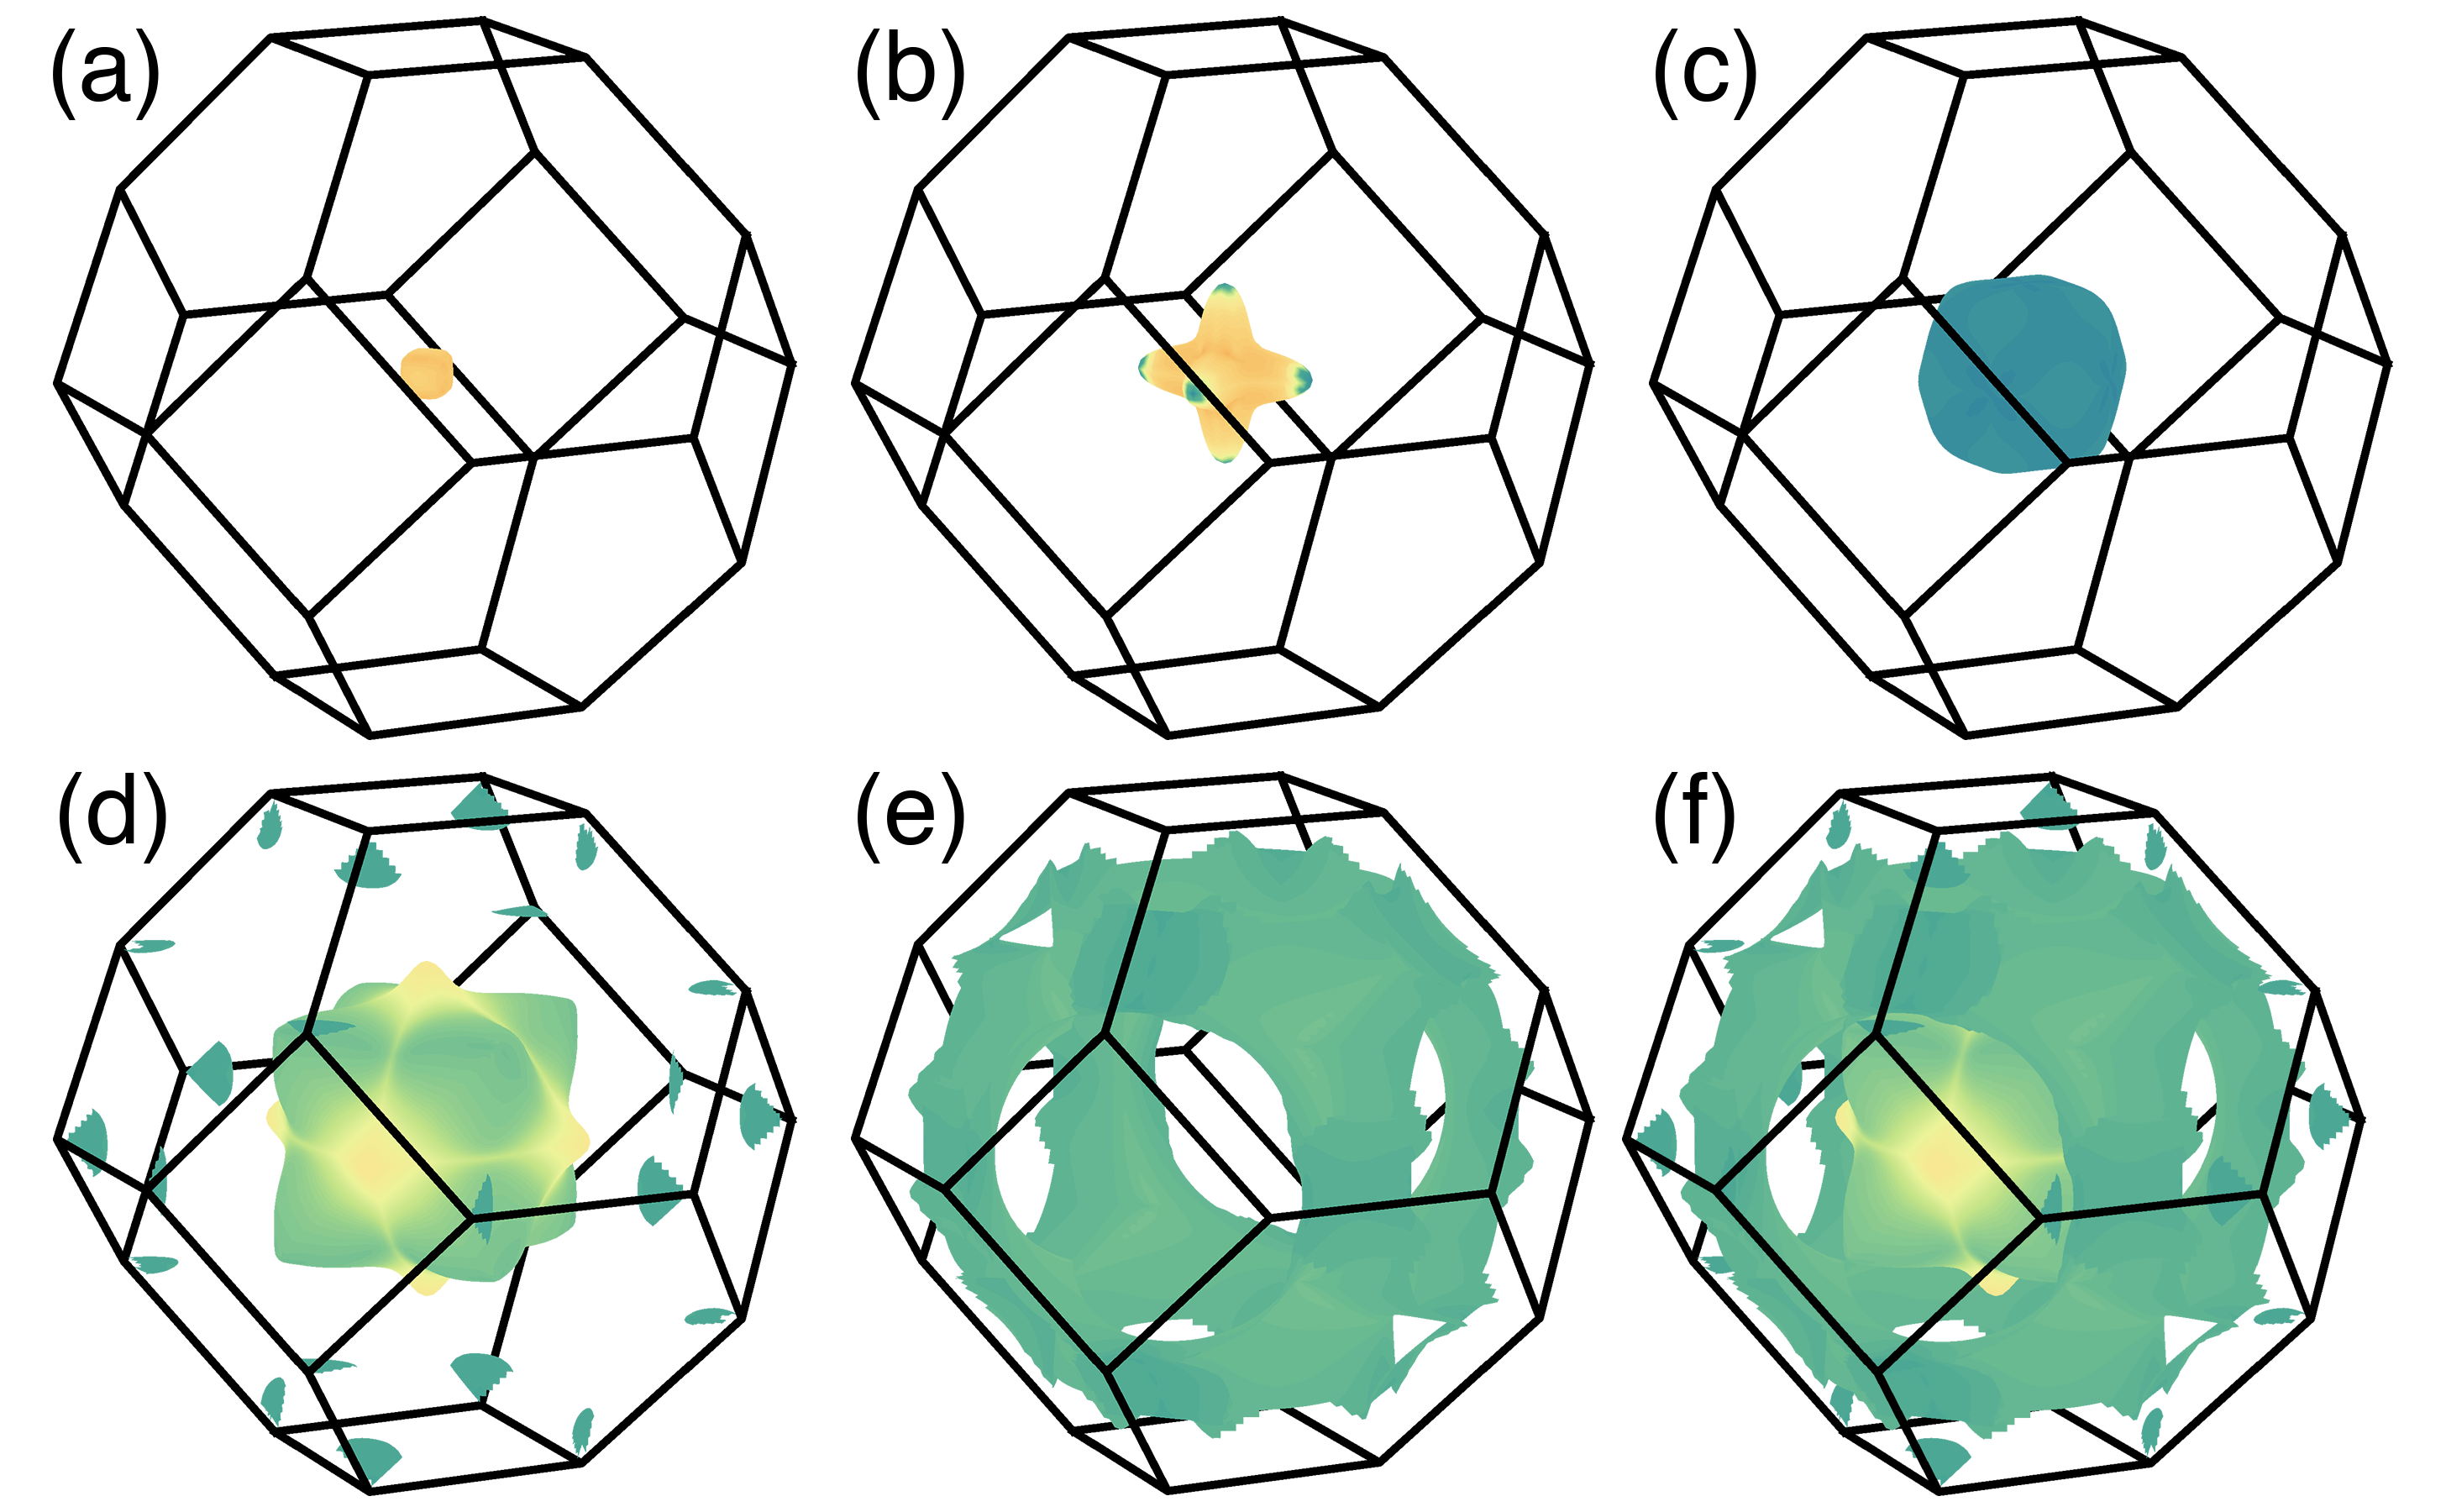
\includegraphics[width=0.47\textwidth]{Figure_2_fermi_surface.png}
\caption[LRC circuit response.]{\label{fig:fermi_surface} }
\end{figure}

The Fermi surface topology determines the phase space available for phonon-assisted electronic scattering and, conversely, electron-screened phonon softening. Because the vibrational energies are orders of magnitudes lower than electronic band widths, the energies that phonons supply to scattered electrons is negligible and, therefore, scattering amounts to simply rearranging electrons on the Fermi surface. The rate at which phonons with momenta $\hbar\vec{q}$ scatter electrons is directly proportional to the overlap area produced by the Fermi surface and it's $\vec{q}$-displaced image. The quantity characterizing the phase space is called the Fermi surface nesting function, 
%
\begin{equation}
\label{eq:nesting}
\nesting = \int \delta\big[ E(\vec{k}) - E_F \big] \delta\big[ E(\vec{k + q}) - E_F \big] d\vec{k},
\end{equation}
%
and its value on the plane containing $\mathrm{[001]}$ and $\mathrm{[110]}$ are plotted in Figure \ref{fig:nesting_2d}. The midpoint of each facet where $\nesting$ peaks in intensity corresponds to the zone center. As the distance from $\Gamma$ is increased $\nesting$ decreases. The rate of decay depends along the crystallographic orientation. The slow decay along $\Delta$ is attributed to the $d_{eg}$ star-like states which exhibit prongs along $\mathrm{[001]}$ directions. 

Between $XK$ the $\nesting$ displays a pronounced increase above background. 

Along the Brillouin zone boundary, 

As the long-wavelenth limit is approached, $\nesting$ diverges 


%
\begin{figure}[h]
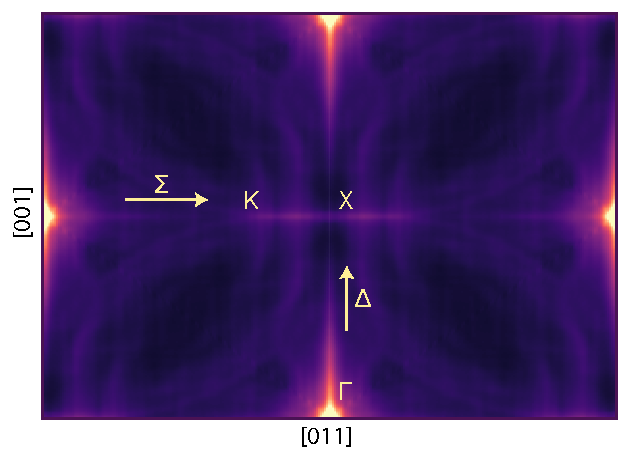
\includegraphics[width=0.47\textwidth]{Figure_3_nesting_2d.pdf}
\caption[LRC circuit response.]{\label{fig:nesting_2d} }
\end{figure}

Figure \ref{fig:nesting_1d} shows the nesting function along high symmetry reciprocal space directions.
\begin{figure}[h]
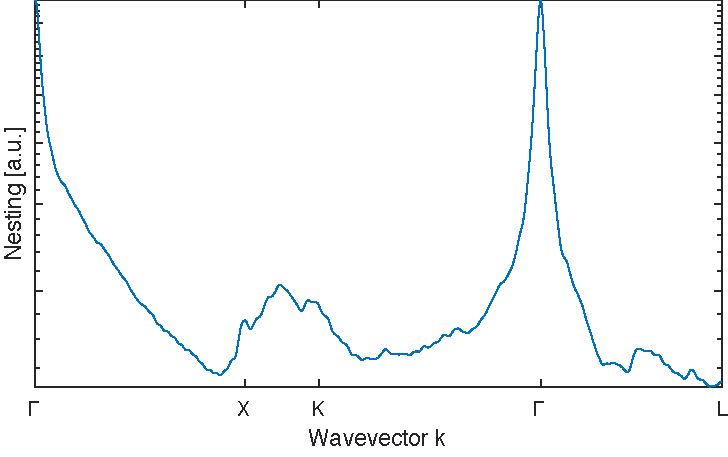
\includegraphics[width=0.47\textwidth]{Figure_4_nesting_1d.pdf}
\caption[LRC circuit response.]{\label{fig:nesting_1d} }
\end{figure}






\section{Hamiltonian}

a minimal tight binding basis is employed. 
\begin{equation}
\big[ p_{x}, p_{y}, p_{z}, d_{xz}, d_{xy}, d_{yz}, d_{x^2-y^2}, d_{z^2}	\big]
\end{equation}





The momentum-dependent Hamiltonian
% KITTEL p 247
\begin{align}
\label{eq:matrix_element}
\ham(\vec{k}) = \sum_j \ham(\vec{r}) e^{-i \vec{k}\cdot\vec{r}_{ij}} .
\end{align}
%
$\bondvec \equiv \vec{r}_i - \vec{r}_j$ represents the bond between primitive atom $i$ and its $j^{\textrm{th}}$ neighbor. The matrix elements of $\ham(\vec{r})$, i.e. energy integrals $\braket{\vec{r},i\alpha | \ham | \vec{r},j\beta}$, are called on-site energies when $i=j$ and hopping terms otherwise. Together, they represent the tight-binding parameters and completely specify the electronic band dispersion. 


Character representation theory (Appendix \ref{appendix:groups}) is employed to identify symmetry-adapted matrix-elements describing on-site orbital energies. 

On-site energies are subject to the full point group symmetry of the NaCl lattice. In descending from the three-dimensional orthogonal group $O(3)$ to the crystallographic point group $O_h$, the three-fold degeneracy of $p$ orbitals is preserved as $T_{1u}$ a triply-degenerate irreducible representation. As a result, matrix elements between $p$ orbitals transform as $T_{1u} \otimes T_{1u} = [A_{1g} \oplus E_g \oplus T_{2g}] \oplus \{T_{1g}\}$, with terms in square and curly brackets corresponding to symmetric and antisymmetric components.\footnote{In the $p$ basis, $T_{1g}$ and $T_{2g}$ are three-dimensional matrices with nonzero elements at off-diagonal positions; $E_g$ is a traceless matrix with nonzero elements at diagonal positions; and $A_{1g}$ is the identity matrix. Basis functions for $T_{1g}$, $T_{2g}$, $E_g$, and $A_{1g}$ include $\ket{x}\bra{y} - \ket{y}\bra{x}$, $\ket{x}\bra{y} + \ket{y}\bra{x}$, $\ket{x}\bra{x} + e^{i2\pi/3}\ket{y}\bra{y} + e^{-i2\pi/3}\ket{z}\bra{z}$, and $\ket{x}\bra{x} + \ket{y}\bra{y} + \ket{z}\bra{z}$, respectively.} The \emph{sole} occurrence of identity irreducible representation $A_{1g}$ in the decomposition signifies the existence \emph{one} symmetry-adapted tight-binding parameter, which is identified as the energy of the triply-degenerate $p$ states
%
\begin{align}
\begin{split}
b_1=\braket{p_x|\ham|p_x}=\braket{p_y|\ham|p_y}=\braket{p_z|\ham|p_z}.
\end{split}
\end{align}
%

$O_h$ lifts the five-fold degeneracy of V 3$d$ producing a two-dimensional $E_g$ and a three-dimensional $T_{2g}$ irreducible representation. The outer product $E_g \otimes E_g$ decomposes into $[A_{1g} \oplus E_g] \oplus \{A_{2g}\}$; $T_{2g} \otimes T_{2g}$ factors into $[A_{1g} \oplus E_{g} \oplus T_{2g}] \oplus \{T_{1g}\}$; and $T_{2g} \otimes E_g$ reduces to $T_{1g} \oplus T_{2g}$. One identity representations occurs in the decomposition of each of the mutual products indicating the existence of two independent energies associated with V 3$d$ $E_g$ and $T_{2g}$ states:
%
\begin{align}
\begin{split}
a_1&\equiv\braket{d_{xy}|\ham|d_{xy}}=\braket{d_{yz}|\ham|d_{yz}}=\braket{d_{zx}|\ham|d_{zx}}\\
a_2&\equiv\braket{d_{z^2}|\ham|d_{z^2}}=\braket{d_{x^2-y^2}|\ham|d_{x^2-y^2}}\\
\end{split}
\end{align}
%
The energy difference $\Delta = a_2 - a_1$ is the crystal field splitting energy. 

On-site interactions ($\vec{r}_{ij} = 0$) produce dispersionless energy integrals exhibiting bands which are independent of wavevector $\vec{k}$ (Eq. \ref{eq:matrix_element}). The inclusion of neighbor interactions, associated with finite bond vectors (i.e., $\vec{r}_{ij} \neq 0$), introduces nontrivial Fourier components and contribute hopping elements to the Hamiltonian that modulate band energies throughout the Brillouin zone. In order to determine irreducible hopping parameters, explicit symmetry relations are identified between off-site matrix elements using crystallographic symmetries, orbital translational properties, and group-theoretical analyses (Appendices \ref{appendix:groups} and \ref{appendix:symmetries}). 


\todo{make use of the group generators in this discussion}











$d$ states factor as $E_g \rightarrow A_1 \oplus B_1$ and $T_{2g} \rightarrow B_2 \oplus E$, $p$ states reduce as $T_{1u} \rightarrow A_1 \oplus E$. Since nonvanishing hopping parameters occur only twice for the identity-containing products $A_1 \otimes A_1 = A_1$ and $E \otimes E = [ A_1 \oplus B_1 \oplus B_2 ] \oplus \{ A_2 \}$, two matrix elements are independent. Two are found to be dependent and the remaining eleven are identified as nil. The nonzero parameters are determined from symmetry relations enforced by Eq.\ref{eq:commutator}:

fist neighbor V-N. 15 possible matrix elements; 11 are zero; two out of the four are independent.
%
\begin{align}
\begin{split}
c_1 & \equiv \braket{p_{x}|\ham|d_{xz}} = -\braket{p_{y}|\ham|d_{yz}} \\
c_2 & \equiv \braket{p_{z}|\ham|d_{x^2-y^2}} = \braket{p_{z}|\ham|d_{z^2}}/\sqrt{3} 
\end{split}
\end{align}

V-V second-neighbors (bond [011]); 15 possible matrix elements, matrix elements between $d_{xz}$, $d_{xy}$ and $d_{yz}$, $d_{x^2-y^2}$, and $d_{z^2}$ are zero (total of six); of remaining 9, six are independent:
%
\begin{align}
\begin{split}
d_1 & \equiv \braket{d_{xy}|\ham|d_{xz}} = \braket{d_{xz}|\ham|d_{xy}} \\
d_2 & \equiv \braket{d_{xz}|\ham|d_{xz}} = \braket{d_{xy}|\ham|d_{xy}} \\
d_3 & \equiv \braket{d_{yz}|\ham|d_{yz}} \\
d_4 & \equiv 2\braket{d_{z^2}|\ham|d_{x^2-y^2}}/\sqrt{3} \\
d_5 & \equiv \braket{d_{x^2-y^2}|\ham|d_{yz}} = -\braket{d_{z^2}|\ham|d_{yz}}/\sqrt{3} \\
d_6 & \equiv \braket{d_{x^2-y^2}|\ham|d_{x^2-y^2}} - 2\braket{d_{x^2-y^2}|\ham|d_{z^2}}/\sqrt{3}
\end{split}
\end{align}


N-N second-neighbors; six possible matrix elements, two are zero (between x and y or z). of the remaining four, three are independent:
%
\begin{align}
\begin{split}
e_1 & \equiv \braket{p_{x}|\ham|p_{x}} \\
e_2 & \equiv \braket{p_{y}|\ham|p_{z}} \\
e_3 & \equiv \braket{p_{y}|\ham|p_{y}} = \braket{p_{z}|\ham|p_{z}} \\
\end{split}
\end{align}

Closed-form expressions for the Hamiltonian are provided in the Appendix.

\section{Acknowledgements}

\bibliography{library}
\clearpage
\appendix

%%
%% WIGNER D MATRIX
%%
%\section{wigner D matrix} 
%\label{appendix:wigner}
%
%In terms of Tait-Bryan angles:
%%
%\footnote{
%Conversion of $3\x3$ transformation matrices $R = R_x(\theta)R_y(\phi)R_z(\gamma)$ to Tait-Bryan angles $\theta$, $\phi$, and $\gamma$ representing rotations about $\hat{z}$, $\hat{y}$, and $\hat{x}$ axes is achieved via:
%\begin{equation}
%\theta = {\rm atan2}(R_{23},R_{33})
%\end{equation}
%\begin{equation}
%\phi   =-{\rm atan2}(-R_{13},\sqrt{R_{11}^2+R_{12}^2})
%\end{equation}
%\begin{equation}
%\begin{split}
%\gamma =-{\rm atan2}(R_{31}\sin{\theta}-R_{21}\cos{\theta}, \\ 
%       \quad         R_{22}\cos{\theta}-R_{32}\sin{\theta})
%\end{split}
%\end{equation}
%${\rm atan2}$ is the four-quadrant arctangent function and $R_{ij}$ are the elements $ij$ of $R$. This formulation avoids gimbal lock.} 
%%
%\begin{equation}
%\wignerDl = e^{-i\theta\hat{L}_x/\hbar} e^{-i\phi\hat{L}_y/\hbar} e^{-i\psi\hat{L}_z/\hbar}
%\end{equation}
%%
%in which angular momentum operators:
%%
%\footnote{For numerical stability, the exponentiated operators are evaluated using the property: \abmei{XX} } \cite{shankar_fundamentals_2014}
%%
%\begin{align}
%\label{eq:angular_momenta}
%% x y z <- z x y
%% Shankar p 327-328, Eq. 12.5.21a-b
%% Wolfram p 85-87
%\hat{L}_x & = \hbar (\hat{L}_{+}-\hat{L}_{-})/2i \\
%\hat{L}_y & = \hbar (\hat{L}_{+}+\hat{L}_{-})/2  \\
%\hat{L}_z & = \hbar m \delta_{l,l'}\delta_{m,m'}
%\end{align}
%$\hat{L}_+$ and $\hat{L}_-$ are raising and lowering operators, with matrix elements:
%\begin{equation}
%\label{eq:raising_lowering_operator}
%% Shankar p 327, Eq. 12.5.20
%\hat{L}_{\pm} = \delta_{l,l'}\delta_{m\pm1,m'} \sqrt{(l\mp m)(l\pm m+1)},
%\end{equation}
%
%
%
%
%
%
%
%
%
%The conversion from spherical to cubic harmonics, $\ket{lm} \rightarrow \ket{\alpha}$, is achieved by conjugating $\wignerDl$ with:
%\begin{equation}
%\label{eq:cubic_harmonics}
%Y_{lm} = 
%\begin{cases}
%  [(-1)^{m}\delta_{ mm'}+\delta_{-mm'}]/\sqrt{2} & \text{if } m < 0 \\
%\delta_{mm}                                      & \text{if } m = 0 \\
% i[(-1)^{m}\delta_{-mm'}-\delta_{ mm'}]/\sqrt{2} & \text{if } m > 0
%\end{cases}
%\end{equation}
%
%
%
%
%
%
%
%
%%\section{Film growth and characterization}
%
%\section{$O_h$}
%\label{appendix:pg}
%\section{Calculation of irreducible characters}
%\label{appendix:chartab}
%Characters $\chi_{i\mu}$ corresponding to irreducible representation $\Gamma_\mu$ and class $\class_i$ are determined using the Burnside algorithm.\cite{burnside_theory_2010,mckay_construction_1970,unger_computing_2006,schneider_dixons_1990,dixon_high_1967} In this approach, class products are decomposed into class sums:
%\begin{equation}
%\label{eq:class_coefficients}
%\class_i \class_j = \sum_k h_{jk}^{(i)} \class_k
%\end{equation}
%with $h_{jk}^{(i)}$ being the frequency at which $\class_k$ appears in the multiplication of classes $\class_i$ and $\class_j$. The collection of class coefficient matrices $h^{(i)}$ are then simultaneously diagonalized using a matrix pencil approach, producing eigenvalues $\lambda_{i\mu}$ from which the dimensions of irreducible representations
%\begin{equation}
%\label{eq:irrep_dimension}
%d_\mu = \sqrt{ \frac{|g|}{\sum_i \lambda_{i\mu} \lambda^{\dag}_{i\mu} / n_i }  }
%\end{equation}
%and their characters
%\begin{equation}
%\label{eq:irrep_characters}
%\chi_{i\mu} = \frac{d_\mu \lambda_{i\mu}}{n_i}
%\end{equation}
%are computed. $n_i$ and $|g|$ are the number of elements in the class $i$ and the group. Elements in the same class have the same character.
%
%Reduction coefficients $n_\mu$, defined as the number of times an irreducible representation $\Gamma^\mu$ appears in a reducible representation $\Gamma$:
%\begin{equation}
%\label{eq:irrep_decomposition}
%\Gamma = \bigoplus_\alpha n_\alpha \Gamma_{i\alpha}
%\end{equation}
%are obtained from:
%\begin{equation}
%\label{eq:irrep_decomposition_coefficients}
%% Wolfram p 20
%n_\alpha = \frac{1}{|g|} \sum_i \chi\left(\Gamma_{i\alpha}\right)^\dag \chi\left(\Gamma_i\right)
%\end{equation}
%The sum is over classes $i$, with number of elements $h_i$, and characters corresponding to the $\alpha$ irreducible representation $\chi(\Gamma_i^\alpha)$.


% - - - - - - - - - - - - - - - - - - - - - - - - - - - - - - - - - - - - - - - - - - - - - - - - - - - - - - - - - - - -
% - - - - - - - - - - - - - - - - - - - - - - - - - - - - - - - - - - - - - - - - - - - - - - - - - - - - - - - - - - - -


\section{\label{appendix:groups} B1 NaCl-structure VN}

The B1 NaCl-structure VN primitive lattice is defined by basis vectors 
%
\begin{align}
\begin{split}
a_1 &= a_o (\hat{y} + \hat{z})/2 \\
a_2 &= a_o (\hat{z} + \hat{x})/2 \\ 
a_3 &= a_o (\hat{x} + \hat{y})/2	
\end{split}
\end{align}
%
with relaxed-lattice parameter $a_o = 0.4134$ nm. The primitive cell contains one V cation and one N anion at $\vec{r}_V = a_o[000]$ and $\vec{r}_N = a_o[\frac{1}{2}\frac{1}{2}\frac{1}{2}]$.  

The point group of the NaCl-structure lattice is the non-Abelian group $O_h$(m$\bar{3}$m). $O_h$(m$\bar{3}$m) contains forty-eight symmetry operations. Twenty-four are proper rotations belonging to the chiral octahedral subgroup $O$(432) and may be further subdivided among five conjugacy classes\footnote{Classes $\class_i$ are mutually distinct sets containing symmetries $R_i$ and $R_j$ related by conjugation with $R_k$ an arbitrary group element: $R_kR_iR_k^{-1}=R_j$}: $\id$, $3c_4^2$, $6c_2$, $8c_3$, and $6c_4$, which correspond to the identity, two-fold rotations about $\left<001\right>$, two-fold rotations around $\left<011\right>$, three-fold rotations about $\left<111\right>$, and four-fold rotations around $\left<001\right>$. The additional twenty-four symmetries are improper rotations formed by compounding $O$ symmetries with the inversion operator $i$ and may be further categorized in five conjugacy classes -- $i$, $3\sigma_2$, $6\sigma_2$, $8\sigma_6$, and $6\sigma_4$ -- associated with inversion, reflection across $\{001\}$, reflection across $\{011\}$, three-fold roto-inversions around $\left<111\right>$, and four-fold roto-inversions about $\left<001\right>$. The $O_h$(m$\bar{3}$m) group has two generators, \footnote{The generating basis of a group is a minimal set of elements which is capable of producing all elements in the group when multiplied together.} $c_4$ and $\sigma_6$.


Beyond the primitive cell, the NaCl-structure lattice can be represented as two interpenetrating V cation and N anion face-centered cubic sublattices displaced by half a primitive cell. Each cation (anion) has six equivalent first neighbor anions (cations) at $\bondvec = a_o [0 0 \frac{1}{2}]$ and twelve second neighbor cations (anions) at $\bondvec = a_o[0 \frac{1}{2} \frac{1}{2}]$. 

First-neighbor bonds $\bondvec = a_o[00\frac{1}{2}]$ are left invariant (i.e., stabilized) by symmetries belonging to the $O_h$ subgroup $C_{4v}$(4mm). These include the identity $\id \seitz{1}{0}$ as well as a two-fold $c_{4}^2$ and two four-fold $c_{4}$ rotations around $\bondvec$: $\seitz{2_{001}}{0}$, $\seitz{2_{001}}{0}$, $\seitz{4^-_{001}}{0}$, and $\seitz{4^+_{001}}{0}$. In addition, there are four mirror planes, of which two are vertical $\sigma_v$, $\seitz{m_{010}}{0}$ and $\seitz{m_{100}}{0}$, and two are diagonal $\sigma_d$, $\seitz{m_{\frac{1}{2}\bar{\frac{1}{2}}0}}{0}$ and $\seitz{m_{\frac{1}{2}\frac{1}{2}0}}{0}$; the intersection of the mirror planes contains $\bondvec$. $c_4$ and $\sigma_v$ form the generating basis of $C_{4v}$(4mm). Coset representatives, which multiply subgroup symmetries to regenerate the $O_h$ parent group, are XXX.\todo{add:coset reps}

Second-neighbor bonds $\bondvec = a_o[0\frac{1}{2}\frac{1}{2}]$ are stabilized by $C_{2v}$(2mm) subgroup elements: the identity $\id \seitz{1}{0}$, two-fold rotation $c_2 \seitz{ 2_{0\frac{1}{2}\frac{1}{2}} }{0}$, vertical-mirror plane $\sigma_v \seitz{m_{001}}{0}$, and diagonal-mirror plane $\sigma_d \seitz{m_{0\frac{1}{2}\bar{\frac{1}{2}}}}{0}$ -- the latter two are generators.

%The $O_h$ point group has twelve $C_{2v}$ subgroups. Six belong to the intermediate subgroup of $C_{4v}$ and six are maximal subgroups of $O_h$.\cite{wadhawan_introduction_2000} The proper choice of subgroup affects the the subduction of $O_h$ irreducible representations onto the .

Irreducible characters belonging to $O_h$(m$\bar{3}$m) and $C_{4v}$, $C_{2v}$, and $C_{3v}$ subgroups are computed using the Burnside algorithm; results are summarized in Table \ref{table:chartab} in accordance with Mulliken\footnote{In Mulliken notation, letters A,E,G, and H denote irreducible representations of dimensions one, two, three, and four. B is used in lieu of A for symmetries which are antisymmetric with respect to the principal axis (the axis of highest cyclical symmetry). Subscripts pairs $g$ and $u$, $1$ and $2$ as well as single and double primes are used to denote representations displaying even and odd parities with respect to inversion, horizontal two-fold rotations $c_2$, and horizontal reflections $\sigma_h$.} and BSW notations. Also shown in Table \ref{table:chartab} are the irreducible characters of $p$ and $d$ tesseral harmonics, the direct sum $p \oplus d$, and of the outer products $p \otimes p$, $p \otimes d$, and $d \otimes d$. Tesseral harmonics are irreducible representations of the three-dimensional orthogonal group $O(3)$, which describe the combination of all possible unitary rotations and reflections in three dimensions. 

Using the irreducible characters in Table \ref{table:chartab}, Subduced representations of $O_h$ onto its subgroups are determined and the results summarized in Table \ref{table:subduction}. \todo{add what subduction and irreducible characters mean}

%
\begin{table}
\caption{\label{table:chartab} Character Tables}
\begin{ruledtabular}
\begin{tabular*}{10cm}{llrrrrrrrrrr}
\multicolumn{2}{c}{$O_h$}         &$\id$&3$c_4^2$& 6$c_2$ & 8$c_3$ & 6$c_4$ &  $i$ & 3$\sigma_2$ & 6$\sigma_2$ & 8$\sigma_6$ & 6$\sigma_4$ \\  
\hline
$A_{1g}$        & $\Gamma_{1}  $  &  1  &     1  &     1  &     1  &     1  &   1  &          1  &          1  &          1  &          1  \\         %  irrep =  1 
$A_{2g}$        & $\Gamma_{2}  $  &  1  &     1  &    -1  &     1  &    -1  &   1  &          1  &         -1  &          1  &         -1  \\         %  irrep =  2 
$E_g   $        & $\Gamma_{12} $  &  2  &     2  &     0  &    -1  &     0  &   2  &          2  &          0  &         -1  &          0  \\         %  irrep =  3 
$T_{1g}$        & $\Gamma_{15} $  &  3  &    -1  &    -1  &     0  &     1  &   3  &         -1  &         -1  &          0  &          1  \\         %  irrep =  5 
$T_{2g}$        & $\Gamma_{25} $  &  3  &    -1  &     1  &     0  &    -1  &   3  &         -1  &          1  &          0  &         -1  \\         %  irrep =  4 
$A_{1u}$        & $\Gamma_{1} '$  &  1  &     1  &     1  &     1  &     1  &  -1  &         -1  &         -1  &         -1  &         -1  \\         %  irrep =  7 
$A_{2u}$        & $\Gamma_{2} '$  &  1  &     1  &    -1  &     1  &    -1  &  -1  &         -1  &          1  &         -1  &          1  \\         %  irrep =  6 
$E_u   $        & $\Gamma_{12}'$  &  2  &     2  &     0  &    -1  &     0  &  -2  &         -2  &          0  &          1  &          0  \\         %  irrep =  8 
$T_{1u}$        & $\Gamma_{15}'$  &  3  &    -1  &    -1  &     0  &     1  &  -3  &          1  &          1  &          0  &         -1  \\         %  irrep =  9 
$T_{2u}$        & $\Gamma_{25}'$  &  3  &    -1  &     1  &     0  &    -1  &  -3  &          1  &         -1  &          0  &          1  \\ \hline \hline %  irrep = 10 
\multicolumn{2}{c}{$C_{4v}$}      &$\id$& $c_4^2$&        &        & 2$c_4$ &      & 2$\sigma_v$ &  $\sigma_d$ &             &             \\ 
\hline
$A_1$           & $\Delta_{1}  $  &  1  &     1  &     .  &     .  &     1  &   .  &          1  &          1  &          .  &          .  \\         %  irrep =  1
$A_2$           & $\Delta_{1}' $  &  1  &     1  &     .  &     .  &     1  &   .  &         -1  &         -1  &          .  &          .  \\         %  irrep =  4
$B_1$           & $\Delta_{2}  $  &  1  &     1  &     .  &     .  &    -1  &   .  &          1  &         -1  &          .  &          .  \\         %  irrep =  3
$B_2$           & $\Delta_{2}' $  &  1  &     1  &     .  &     .  &    -1  &   .  &         -1  &          1  &          .  &          .  \\         %  irrep =  2
$E$             & $\Delta_{5}  $  &  2  &    -2  &     .  &     .  &     0  &   .  &          0  &          0  &          .  &          .  \\ \hline \hline %  irrep =  5
\multicolumn{2}{c}{$C_{2v}$}      &$\id$&        &  $c_2$ &        &        &      &  $\sigma_v$ & $\sigma_d$  &             &             \\
\hline
$A_{1}$         & $\Sigma_{1}  $  &  1  &     .  &     1  &     .  &     .  &   .  &          1  &          1  &          .  &          .  \\
$A_{2}$         & $\Sigma_{2}  $  &  1  &     .  &     1  &     .  &     .  &   .  &         -1  &         -1  &          .  &          .  \\
$B_{1}$         & $\Sigma_{3}  $  &  1  &     .  &    -1  &     .  &     .  &   .  &         -1  &          1  &          .  &          .  \\
$B_{2}$         & $\Sigma_{4}  $  &  1  &     .  &    -1  &     .  &     .  &   .  &          1  &         -1  &          .  &          .  \\ \hline \hline
\multicolumn{2}{c}{$C_{3v}$}      &$\id$&        &        & 2$c_3$ &        &      &             & 3$\sigma_v$ &             &             \\
\hline
$A_{1}$         & $\Lambda_{1} $  &  1  &     .  &     .  &     1  &     .  &   .  &          .  &          1  &          .  &          .  \\
$A_{2}$         & $\Lambda_{2} $  &  1  &     .  &     .  &     1  &     .  &   .  &          .  &         -1  &          .  &          .  \\
$E$             & $\Lambda_{3} $  &  2  &     .  &     .  &    -1  &     .  &   .  &          .  &          0  &          .  &          .  \\ \hline \hline
\multicolumn{2}{c}{$p$          } &  3  &     -1 &    -1  &     0  &     1  &  -3  &          1  &          1  &          0  &         -1  \\
\multicolumn{2}{c}{$d$          } &  5  &      1 &     1  &    -1  &    -1  &   5  &          1  &          1  &         -1  &         -1  \\
\multicolumn{2}{c}{$p \oplus  d$} &  8  &      0 &     0  &    -1  &     0  &   2  &          2  &          2  &         -1  &         -2  \\
\multicolumn{2}{c}{$p \otimes p$} &  9  &      1 &     1  &     0  &     1  &   9  &          1  &          1  &          0  &          1  \\
\multicolumn{2}{c}{$p \otimes d$} & 15  &     -1 &    -1  &     0  &    -1  & -15  &          1  &          1  &          0  &          1  \\
\multicolumn{2}{c}{$d \otimes d$} & 25  &      1 &     1  &     1  &     1  &  25  &          1  &          1  &          1  &          1  \\
\end{tabular*}
\end{ruledtabular}
\end{table}
%
\begin{table}
\caption{\label{table:subduction} $O_h$ subductions}
\begin{ruledtabular}
\begin{tabular*}{10cm}{llll}
$O_h$    & $C_{4v}$         & $C_{2v}$                              &   $C_{3v}$            \\ \hline
$A_{1g}$ & $A_1$            & $A_{1}$                               &   $A_1$               \\ 
$A_{2g}$ & $B_1$            & $B_{1}$                               &   $A_2$               \\ 
$E_g   $ & $A_1 \oplus B_1$ & $A_{1} \oplus B_{1}$                  &   $E$                 \\ 
$T_{1g}$ & $A_2 \oplus E$   & $A_{2} \oplus B_{1} \oplus B_{2}$     &   $A_2 \oplus E$      \\ 
$T_{2g}$ & $B_2 \oplus E$   & $A_{1} \oplus A_{2} \oplus B_{2}$     &   $A_1 \oplus E$      \\ 
$A_{1u}$ & $A_2$            & $A_{2}$                               &   $A_2$               \\ 
$A_{2u}$ & $B_2$            & $B_{2}$                               &   $A_1$               \\ 
$E_u   $ & $A_2 \oplus B_2$ & $A_{2} \oplus B_{2}$                  &   $E$                 \\ 
$T_{1u}$ & $A_1 \oplus E$   & $A_{1} \oplus B_{1} \oplus B_{2}$     &   $A_1 \oplus E$      \\ 
$T_{2u}$ & $B_1 \oplus E$   & $A_{1} \oplus A_{2} \oplus B_{1}$     &   $A_2 \oplus E$      \\ 
\end{tabular*}
\end{ruledtabular}
\end{table}

% - - - - - - - - - - - - - - - - - - - - - - - - - - - - - - - - - - - - - - - - - - - - - - - - - - - - - - - - - - - -
% - - - - - - - - - - - - - - - - - - - - - - - - - - - - - - - - - - - - - - - - - - - - - - - - - - - - - - - - - - - -

\section{\label{appendix:symmetries} Transformations and Symmetries}
Transformational properties and symmetry relations for identifying irreducible tight-binding parameters are presented. 

Abstract operations $\hat{R}$ become concrete representations which depend on the object being described. Rotation of cartesian vectors (or, equivalently, atomic bonds) by proper symmetries may be represented as $ R \vec{r} \rightarrow \vec{r} '$, in which $R$ are $3\times3$ rotation matrix. Analogously, the action of $\hat{R}$ on atomic-like orbitals may be represented as $\wignerDl\ket{i\alpha} \rightarrow \ket{i\beta}$, in which 
% LAX p 43 Eq 2.5.18
\begin{equation}
\wignerDl = e^{- \theta \hat{n} \cdot \hat{L} /\hbar}
\end{equation}
are Wigner functions \footnote{Wigner functions couple states with different magnetic but equal azimuthal quantum numbers and, as a result, cannot alter orbital characters, i.e. transform $p$ states into $d$ states.}, ($2l$+$1$)-dimensional unitary square matrices which parameterize proper rotations via the angular momentum operator $\hat{L}$, angle $\theta$, and axis $\hat{n}$. $\hbar$ is Planck's reduced constant and $l$ is the orbital's azimuthal quantum number. Improper transformations are realized by multiplying proper representations with $(-1)^l$, the scalar inversion operator.\cite{sharma_general_1979,el-batanouny_symmetry_2008} % WOOOTEN p 604 after Eq. 14.164

In transforming state-vectors (Eq. \ref{eq:statevec}), $\hat{R}$ incarnates as $\wignerD$: $\wignerD \ket{\psi} \rightarrow \ket{\psi'}.$ $\wignerD$ combines the effects of permuting atoms onto their equivalents and of coupling the magnetic quantum numbers of atomic-like orbitals. In the absence of the permutations, $\wignerD$ simplifies to a direct sum over Wigner functions $\wignerDl$ associated with primitive cell orbitals: $\wignerD = \bigoplus_l \wignerDl$. $\wignerD$ also describes the action of $\hat{R}$ on the Hamiltonian, since the latter transforms as the outer product of state-vectors: $\mathbb{D}^\dag \ham(\vec{r}) \wignerD \rightarrow \ham( R\vec{r})$. \cite{el-batanouny_symmetry_2008} % WOOTEN p 78, Eq. 13.9

Symmetry operations which transform the lattice into indistinguishable configurations leave the Hamiltonian invariant. Invariances associated with space group symmetries are enforced through:
% NYE p 11, Eq. 22
\begin{equation}
\label{eq:stab}
\ham^{\alpha\beta}_{ij}(\vec{r}) = \sum_{\mu\nu} \ham^{\mu\nu}_{ij}(\vec{r}) \mathbb{D}^{\mu\alpha} \mathbb{D}^{\nu\beta},
\end{equation}
which is equivalent to the commutator relationship $[\ham(\vec{r}),\wignerD] = 0$. Invariances associated with the interchange of orbitals positions ($i\alpha \leftrightarrow j\beta$) are described via:
%
\begin{equation}
\label{eq:intrinsic}
\ham^{\alpha\beta}_{ij}(\vec{r}) = (-1)^{l_\alpha+l_\beta} \ham^{\beta\alpha}_{ji}(\vec{r}).
\end{equation}
%
The prefactor arises from orbital parity. The combination of Eqs. \ref{eq:stab} and \ref{eq:intrinsic} completely specify all symmetry relations between tight-binding Hamiltonian matrix elements.

% - - - - - - - - - - - - - - - - - - - - - - - - - - - - - - - - - - - - - - - - - - - - - - - - - - - - - - - - - - - -
% - - - - - - - - - - - - - - - - - - - - - - - - - - - - - - - - - - - - - - - - - - - - - - - - - - - - - - - - - - - -

\begin{widetext}

\section{Explicit Tight-Binding Hamiltonian}

The tight-binding Hamiltonian (Eq. \ref{eq:matrix_element}), evaluated up to second neighbor interactions, is
%
%\begin{widetext}	
%
\begin{align}
\label{eq:ham_explicit}
\ham(\vec{k}) =
\begin{bmatrix}
\ham_{\textrm{V}0}^{dd}(\vec{k}) & 0 \\
0 & \ham_{\textrm{N}0}^{pp}(\vec{k})\\
\end{bmatrix}
+ 
\begin{bmatrix}
0 &\ham_{\textrm{V}1}^{dp}(\vec{k}) \\
\ham_{\textrm{V}1}^{dp}(\vec{k})^{\dagger} & 0 \\
\end{bmatrix}
+ 
\begin{bmatrix}
\ham_{\textrm{V}2}^{dd}(\vec{k}) & 0 \\
0 & \ham_{\textrm{N}2}^{pp}(\vec{k})
\end{bmatrix} .
\end{align}
%
%\end{widetext}
%
$\ham_{ij}^{l_\alpha l_\beta}$ are $(2l_\alpha+1)\times(2l_\beta+1)$-dimensional block matrices which couple orbitals $l_\alpha$ on atom $i$ to orbitals $l_\beta$ on atom $j$. Explicit expressions are provided below.  Because the matrices are Hermitian, only the top half is shown for clarity. Furthermore, trigonometric functions are abbreviated: $c_i = \cos(\pi a k_i)$, $s_i = \sin(\pi a k_i)$, $s_{ij} = s_i s_j$ and $c_{ij} = c_i c_j$, in which $k_i = \vec{k}\cdot\hat{i}$ and $a = 0.4134$ nm is the relaxed VN lattice parameter. On-site energy integrals $\epsilon$ and off-site hopping parameters $v$, optimized by fitting first principles band dispersions computed using density functional theory, are summarized in Table \ref{table:tbparameters}.

%
%%%%%%
%%%%%%
%%%%%%

%%%%%%

\begin{equation}
\label{eq:0pp}
\ham_{\textrm{N0}}^{pp}(\vec{k})=
\begin{bmatrix}
b_{1} & 0     & 0\\
      & b_{1} & 0\\
      &       & b_{1}\\
\end{bmatrix}
\end{equation}
%
\begin{equation}
\label{eq:0dd}
\ham_{\textrm{V0}}^{dd}(\vec{k})=
\begin{bmatrix}
a_{1} & 0     & 0     & 0     & 0\\
      & a_{1} & 0     & 0     & 0\\
      &       & a_{1} & 0     & 0\\
      &       &       & a_{2} & 0\\
      &       &       &       & a_{2}\\
\end{bmatrix}
\end{equation}
%
\begin{equation}
\ham_{\textrm{V1}}^{dp}(\vec{k})=-2i
\begin{bmatrix}
-c_{1}s_{z}        & 0           & -c_{1}s_{x}\\
c_{1}s_{y}         & c_{1}s_{x}  & 0\\
0                  & c_{1}s_{z}  & c_{1}s_{y}\\
-c_{2}s_{x}        & 2c_{2}s_{y} & -c_{2}s_{z}\\
\sqrt{3}c_{2}s_{x} & 0           & -\sqrt{3}c_{2}s_{z}\\
\end{bmatrix}
\end{equation}
%
\begin{equation}
H_2^{dd}=4
\begin{bmatrix}
c_{yz}e_{1}           & \multirow{2}{*}{$-s_{xy}e_{2}$} & \multirow{2}{*}{$-s_{xz}e_{2}$}\\
+(c_{xy}+c_{xz})e_{3} &                                 & \\
\multirow{2}{*}{ }    & c_{xz}e_{1}                     & \multirow{2}{*}{$-s_{yz}e_{2}$}\\
                      & +(c_{xy}+c_{yz})e_{3}           & \\
\multirow{2}{*}{ }    & \multirow{2}{*}{ }              & c_{xy}e_{1} \\
                      &                                 & +(c_{xz}+c_{yz})e_{3}\\
\end{bmatrix}
\end{equation}
%
\begin{equation}
\ham_{\textrm{N2}}^{dd}(\vec{k})=4
\begin{bmatrix}
(c_{xy}+c_{yz})d_{2} & \multirow{2}{*}{$-s_{yz}d_{1}$} & \multirow{2}{*}{$-s_{xy}d_{1}$} & \multirow{2}{*}{$-2s_{xz}d_{5}$} & \multirow{2}{*}{$0$}\\
+c_{xz}d_{3}         &                                 &                                 &                                  & \\
\multirow{2}{*}{ }   & (c_{xz}+c_{yz})d_{2}            & \multirow{2}{*}{$s_{xz}d_{1}$}  & \multirow{2}{*}{$-s_{xy}d_{5}$}  & \multirow{2}{*}{$-\sqrt{3}s_{xy}d_{5}$}\\
                     & +c_{xy}d_{3}                    &                                 &                                  & \\
\multirow{2}{*}{ }   & \multirow{2}{*}{ }              & (c_{xy}+c_{xz})d_{2}            & \multirow{2}{*}{$-s_{yz}d_{5}$}  & \multirow{2}{*}{$\sqrt{3}s_{yz}d_{5}$}\\
                     &                                 & +c_{yz}d_{3}                    &                                  & \\
\multirow{2}{*}{ }   & \multirow{2}{*}{ }              & \multirow{2}{*}{ }              & (c_{xy}-c_{xz}/2+c_{yz})d_{4}    & \multirow{2}{*}{$-\sqrt{3}(c_{xy}-c_{yz})d_{4}/2$}\\
                     &                                 &                                 & +(c_{xy}+c_{xz}+c_{yz})d_{6}     & \\
\multirow{2}{*}{ }   & \multirow{2}{*}{ }              & \multirow{2}{*}{ }              & \multirow{2}{*}{ }               & 3c_{xz}d_{4}/2\\
                     &                                 &                                 &                                  & +(c_{xy}+c_{xz}+c_{yz})d_{6}\\
\end{bmatrix}
\end{equation}
%
\begin{table}[h]
\caption{\label{table:tbparameters} \emph{Ab initio}-optimized NaCl-structure VN tight binding parameters}
% v=[-0.4212,1.1975,-4.1841,-1.0193,-1.0322,-0.0565,0.1132,-0.5218,-0.1680,0.0635,-0.0546,-0.1051,0.4189,0.3061];
\setlength{\tabcolsep}{0.7em} % for the horizontal padding
{\renewcommand{\arraystretch}{1.5}% for the vertical padding
\begin{tabular}{cccccccccccccc}
 $a_{1}$ & $a_{2}$ & $b_{1}$ & $c_{1}$ & $c_{2}$ & $d_{1}$ & $d_{2}$ \\ \hline\hline
 -0.4212 & +1.1975 & -4.1841 & -1.0193 & -1.0322 & -0.0565 & +0.1132 \\
 $d_{3}$ & $d_{4}$ & $d_{5}$ & $d_{6}$ & $e_{1}$ & $e_{2}$ & $e_{3}$ \\ \hline\hline
 -0.5218 & -0.1680 & +0.0635 & -0.0546 & -0.1051 & +0.4189 & +0.3061 \\ 
\end{tabular}
}
\end{table}








\end{widetext}

\end{document}




%
%
% FULL MATRICES
%
%
%
%\begin{equation}
%\label{eq:0pp}
%\ham_{\textrm{N0}}^{pp}(\vec{k})=
%\begin{bmatrix}
%b_{1} & 0     & 0\\
%0     & b_{1} & 0\\
%0     & 0     & b_{1}\\
%\end{bmatrix}
%\end{equation}
%%
%\begin{equation}
%\label{eq:0dd}
%\ham_{\textrm{V0}}^{dd}(\vec{k})=
%\begin{bmatrix}
%a_{1} & 0     & 0     & 0     & 0\\
%0     & a_{1} & 0     & 0     & 0\\
%0     & 0     & a_{1} & 0     & 0\\
%0     & 0     & 0     & a_{2} & 0\\
%0     & 0     & 0     & 0     & a_{2}\\
%\end{bmatrix}
%\end{equation}
%%
%\begin{equation}
%\ham_{\textrm{V1}}^{dp}(\vec{k})=-2i
%\begin{bmatrix}
%-c_{1}s_{z}        & 0           & -c_{1}s_{x}\\
%c_{1}s_{y}         & c_{1}s_{x}  & 0\\
%0                  & c_{1}s_{z}  & c_{1}s_{y}\\
%-c_{2}s_{x}        & 2c_{2}s_{y} & -c_{2}s_{z}\\
%\sqrt{3}c_{2}s_{x} & 0           & -\sqrt{3}c_{2}s_{z}\\
%\end{bmatrix}
%\end{equation}
%%
%\begin{equation}
%H_2^{dd}=4
%\begin{bmatrix}
%c_{yz}e_{1}                     & \multirow{2}{*}{$-s_{xy}e_{2}$} & \multirow{2}{*}{$-s_{xz}e_{2}$}\\
%+(c_{xy}+c_{xz})e_{3}           &                                 & \\
%\multirow{2}{*}{$-s_{xy}e_{2}$} & c_{xz}e_{1}                     & \multirow{2}{*}{$-s_{yz}e_{2}$}\\
%                                & +(c_{xy}+c_{yz})e_{3}           & \\
%\multirow{2}{*}{$-s_{xz}e_{2}$} & \multirow{2}{*}{$-s_{yz}e_{2}$} & c_{xy}e_{1} \\
%                                &                                 & +(c_{xz}+c_{yz})e_{3}\\
%\end{bmatrix}
%\end{equation}
%%
%\begin{equation}
%\ham_{\textrm{N2}}^{dd}(\vec{k})=4
%\begin{bmatrix}
%(c_{xy}+c_{yz})d_{2}             & \multirow{2}{*}{$-s_{yz}d_{1}$}         & \multirow{2}{*}{$-s_{xy}d_{1}$}        & \multirow{2}{*}{$-2s_{xz}d_{5}$}                   & \multirow{2}{*}{$0$}\\
%+c_{xz}d_{3}                     &                                         &                                        &                                                    & \\
%\multirow{2}{*}{$-s_{yz}d_{1}$}  & (c_{xz}+c_{yz})d_{2}                    & \multirow{2}{*}{$s_{xz}d_{1}$}         & \multirow{2}{*}{$-s_{xy}d_{5}$}                    & \multirow{2}{*}{$-\sqrt{3}s_{xy}d_{5}$}\\
%                                 & +c_{xy}d_{3}                            &                                        &                                                    & \\
%\multirow{2}{*}{$-s_{xy}d_{1}$}  & \multirow{2}{*}{$s_{xz}d_{1}$}          & (c_{xy}+c_{xz})d_{2}                   & \multirow{2}{*}{$-s_{yz}d_{5}$}                    & \multirow{2}{*}{$\sqrt{3}s_{yz}d_{5}$}\\
%                                 &                                         & +c_{yz}d_{3}                           &                                                    & \\
%\multirow{2}{*}{$-2s_{xz}d_{5}$} & \multirow{2}{*}{$-s_{xy}d_{5}$}         & \multirow{2}{*}{$-s_{yz}d_{5}$}        & (c_{xy}-c_{xz}/2+c_{yz})d_{4}                      & \multirow{2}{*}{$-\sqrt{3}(c_{xy}-c_{yz})d_{4}/2$}\\
%                                 &                                         &                                        & +(c_{xy}+c_{xz}+c_{yz})d_{6}                       & \\
%\multirow{2}{*}{$0$}             & \multirow{2}{*}{$-\sqrt{3}s_{xy}d_{5}$} & \multirow{2}{*}{$\sqrt{3}s_{yz}d_{5}$} & \multirow{2}{*}{$-\sqrt{3}(c_{xy}-c_{yz})d_{4}/2$} & 3c_{xz}d_{4}/2\\
%                                 &                                         &                                        &                                                    & +(c_{xy}+c_{xz}+c_{yz})d_{6}\\
%\end{bmatrix}
%\end{equation}

